\documentclass[aspectratio=169]{beamer}

% ---------- ENCODING & FONTS ----------
\usepackage[utf8]{inputenc}
\usepackage[T1]{fontenc}

% ---------- THEME & LOOK ----------
\usetheme{Madrid}
\usecolortheme{seahorse}
\usefonttheme{professionalfonts}
\setbeamertemplate{navigation symbols}{}
\setbeamertemplate{footline}[frame number]
\setbeamercovered{transparent}
\setbeamertemplate{itemize items}[circle]
\setbeamertemplate{enumerate items}[default]
\setlength{\parskip}{0.25em}

% ---------- COLORS ----------
\definecolor{accent}{RGB}{0,92,184}
\definecolor{soft}{RGB}{233,244,255}
\definecolor{canadared}{RGB}{196,30,58}
\definecolor{leafgreen}{RGB}{0,130,80}
\definecolor{goldenrod}{RGB}{218,165,32}
\definecolor{deeporange}{RGB}{220,90,20}
\definecolor{shiftpurple}{RGB}{130,50,180}
\definecolor{tealblue}{RGB}{0,128,128}
\setbeamercolor{structure}{fg=accent}
\setbeamercolor{title}{fg=white,bg=accent}
\setbeamercolor{frametitle}{fg=accent}
\setbeamercolor{block title}{bg=accent!12,fg=accent}
\setbeamercolor{block body}{bg=soft}

% ---------- PACKAGES ----------
\usepackage{booktabs}
\usepackage{amsmath, amssymb}
\usepackage{array}
\usepackage{multirow}
\usepackage{hyperref}
\usepackage{tikz}
\usepackage{pgfplots}
\pgfplotsset{compat=1.18}
\usetikzlibrary{arrows.meta, positioning, calc, shapes.geometric}
\hypersetup{colorlinks=true,linkcolor=accent,urlcolor=accent}

% ---------- SAFE TRANSITION FALLBACK ----------
\makeatletter
\@ifundefined{transfade}{\newcommand{\transfade}[1][]{}}{}
\makeatother

% ---------- TITLE ----------
\title{\textbf{GDP: Measuring Total Production and Income}}
\subtitle{{\large ECON 101 -- Principles of Macroeconomics}}
\author{Muhebullah Karimzada}
\date{Spring 2026}

% ============================================================
\begin{document}
% ============================================================

\begin{frame}[plain]
  \titlepage
\end{frame}

\begin{frame}{Chapter Outline}
\transfade
\begin{itemize}[<+->]
  \item \textbf{4.1} Gross Domestic Product Measures Total Production
  \item \textbf{4.2} Does GDP Measure What We Want It to Measure?
  \item \textbf{4.3} Real GDP versus Nominal GDP
  \item \textbf{4.4} Other Measures of Total Production and Total Income
\end{itemize}
\end{frame}

% ============================================================
\section*{Key Macro Concepts}
% ============================================================

\begin{frame}{Some Important Terms in Macroeconomics}
\transfade
\begin{itemize}[<+->]
  \item \textbf{Business cycle:} alternating periods of economic \alert{expansion} and \alert{recession}.
  \item \textbf{Expansion:} total production and employment are \alert{increasing}.
  \item \textbf{Recession:} total production and employment are \alert{decreasing}.
  \item \textbf{Economic growth:} the ability of the economy to produce increasing quantities of goods and services over the long run.
  \item \textbf{Inflation rate:} the \alert{percentage increase} in the price level from one year to the next.
\end{itemize}
\end{frame}

%--- Fig 4.0: Canadian real GDP with business cycle annotation ---
\begin{frame}{Figure 4.0 -- Canada's Real GDP: Business Cycles and Long-Run Growth}
\begin{center}
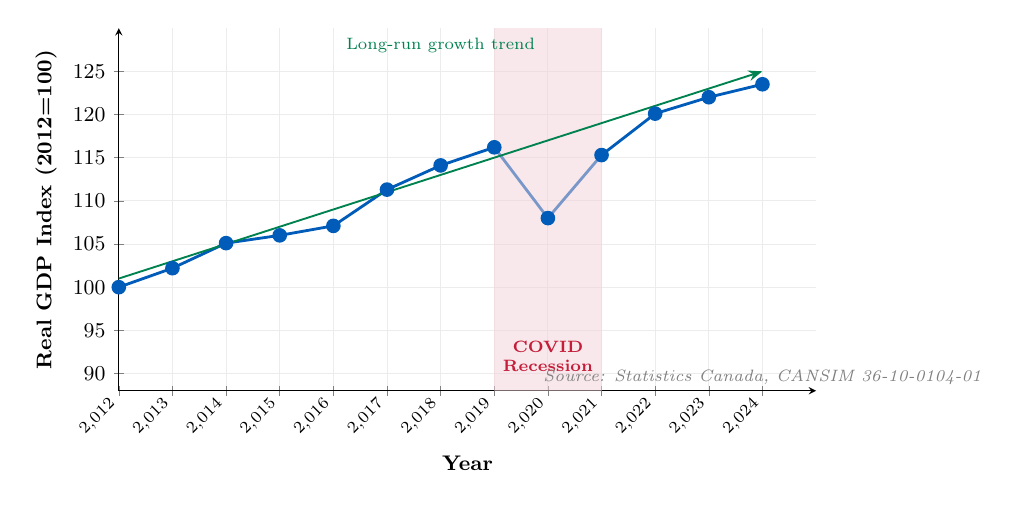
\begin{tikzpicture}[scale=0.85]
  \begin{axis}[
    width=12cm, height=7cm,
    xlabel={\textbf{Year}},
    ylabel={\textbf{Real GDP Index} (2012=100)},
    xmin=2012, xmax=2025,
    ymin=88, ymax=130,
    xtick={2012,2013,2014,2015,2016,2017,2018,2019,2020,2021,2022,2023,2024},
    xticklabel style={rotate=45, anchor=east, font=\scriptsize},
    ytick={90,95,100,105,110,115,120,125},
    tick label style={font=\small},
    label style={font=\small\bfseries},
    axis lines=left,
    grid=major, grid style={gray!15},
    clip=false,
  ]
  % Real GDP index (approx Statistics Canada data, 2012=100)
  \addplot[very thick, color=accent, mark=*, mark size=2.5pt]
    coordinates {
      (2012,100)(2013,102.2)(2014,105.1)(2015,106.0)
      (2016,107.1)(2017,111.3)(2018,114.1)(2019,116.2)
      (2020,108.0)(2021,115.3)(2022,120.1)(2023,122.0)(2024,123.5)
    };
  % Shade recession (COVID)
  \fill[canadared!20, opacity=0.5]
    (axis cs:2019,88) rectangle (axis cs:2021,130);
  \node[font=\scriptsize\bfseries, text=canadared, align=center]
    at (axis cs:2020,92) {COVID\\Recession};
  % Long-run trend arrow
  \draw[-{Stealth[length=6pt]}, thick, color=leafgreen]
    (axis cs:2012,101) -- (axis cs:2024,125);
  \node[font=\scriptsize, text=leafgreen, align=center]
    at (axis cs:2018,128) {Long-run growth trend};
  % Source note
  \node[font=\scriptsize\itshape, text=gray] at (axis cs:2024,89.5)
    {Source: Statistics Canada, CANSIM 36-10-0104-01};
  \end{axis}
\end{tikzpicture}
\end{center}
\end{frame}

\begin{frame}{Why These Concepts Matter for GDP}
\transfade
\begin{itemize}[<+->]
  \item GDP is our main measure of the \textbf{size of the economy}.
  \item Short-run \alert{business cycles} show up as ups and downs in real GDP.
  \item Long-run \alert{economic growth} shows up as an upward trend in real GDP.
  \item Inflation affects \textbf{nominal} GDP, so we must distinguish it from \textbf{real} GDP.
  \item \textbf{Canadian fact:} Canada's nominal GDP reached $\approx$\$3.0 trillion in 2024 (Statistics Canada, CANSIM 36-10-0104-01).
\end{itemize}
\end{frame}

% ============================================================
\section{4.1 Gross Domestic Product Measures Total Production}
% ============================================================

\begin{frame}{4.1 Learning Objective}
\transfade
\begin{block}{Goal}
Explain how total production is measured.
\end{block}
\begin{itemize}[<+->]
  \item \textbf{Gross domestic product (GDP):} the market value of all final goods and services produced in a country during a period of time.
  \item Unpacking the definition:
  \begin{itemize}[<+->]
    \item ``\textbf{market value}'' --- uses prices as a common unit
    \item ``\textbf{final goods and services}'' --- avoids double-counting
    \item ``\textbf{produced in a country}'' --- location matters, not ownership
    \item ``\textbf{during a period of time}'' --- a flow, not a stock
  \end{itemize}
\end{itemize}
\end{frame}

\begin{frame}{``Market Value''}
\transfade
\begin{itemize}[<+->]
  \item We produce many different goods: lumber, canola oil, cars, haircuts, banking services\ldots
  \item We cannot simply add \emph{physical quantities} --- a board-foot of lumber cannot be added to a barrel of oil.
  \item We need a \alert{common unit}: \textbf{money}.
  \item We value each good at its \alert{market price}, giving us the \textbf{market value} of production.
  \item \textbf{Canadian example:} In 2024, one barrel of Western Canadian Select oil $\approx$\$60 CAD; one tonne of potash $\approx$\$340 CAD --- very different physical units, both measured in dollars.
\end{itemize}
\end{frame}

\begin{frame}{Final Goods and Avoiding Double Counting}
\transfade
\begin{itemize}[<+->]
  \item A \textbf{final good or service} is purchased by a final user.
  \item \textbf{Intermediate goods and services} are inputs into other goods.
  \begin{itemize}[<+->]
    \item Example: wheat $\to$ flour $\to$ bread. GDP counts only the final bread sold to consumers.
  \end{itemize}
  \item Counting intermediate goods would cause \alert{double counting}.
  \item \textbf{Canadian example:} Alberta crude oil refined into gasoline sold at the pump --- only the final gasoline sale counts; the crude oil is an intermediate good.
\end{itemize}
\end{frame}

\begin{frame}{``Produced in a Country'' and ``During a Period of Time''}
\transfade
\begin{itemize}[<+->]
  \item GDP measures production within \alert{Canada's borders}, regardless of ownership:
  \begin{itemize}[<+->]
    \item A Toyota plant in Cambridge, ON $\Rightarrow$ \textbf{included} in Canadian GDP.
    \item A Loblaws store in the Bahamas $\Rightarrow$ \textbf{excluded} from Canadian GDP.
  \end{itemize}
  \item GDP is measured for a specific period (a year or quarter):
  \begin{itemize}[<+->]
    \item Only goods \textbf{produced} in that period count.
    \item A used car re-sold in 2025 was already counted when new; it is \textbf{not counted again}.
  \end{itemize}
\end{itemize}
\end{frame}

\begin{frame}{Production = Income: Two Sides of the Same Coin}
\transfade
\begin{itemize}[<+->]
  \item Every dollar of production generates a dollar of \alert{income} for someone:
  \begin{itemize}[<+->]
    \item workers receive \textbf{wages},
    \item capital owners receive \textbf{profit or interest},
    \item landowners receive \textbf{rent}.
  \end{itemize}
  \[
    \text{Total Production} = \text{Total Income}
  \]
  \item This identity underlies both the \textbf{expenditure approach} and the \textbf{income approach} to measuring GDP.
\end{itemize}
\end{frame}

%--- Fig 4.1: Full circular-flow diagram (4 sectors + financial system) ---
\begin{frame}{Figure 4.1 -- The Full Circular-Flow Diagram (Canada)}
\begin{center}
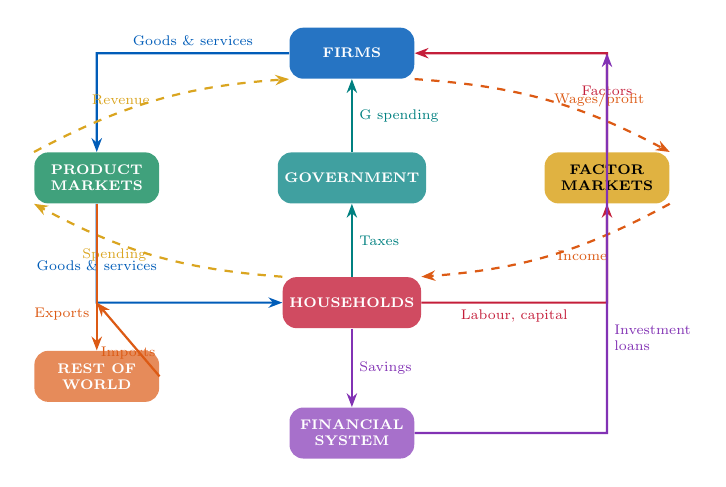
\begin{tikzpicture}[
  box/.style={rectangle, rounded corners=5pt, minimum width=2.2cm,
              minimum height=0.9cm, align=center, font=\scriptsize\bfseries},
  scale=0.72, transform shape
]
  % Main boxes
  \node[box, fill=accent!85, text=white]       (firms) at (0, 2.2)  {FIRMS};
  \node[box, fill=canadared!80, text=white]    (hh)    at (0,-2.2)  {HOUSEHOLDS};
  \node[box, fill=leafgreen!75, text=white]    (prod)  at (-4.5, 0) {PRODUCT\\MARKETS};
  \node[box, fill=goldenrod!85, text=black]    (fact)  at ( 4.5, 0) {FACTOR\\MARKETS};
  \node[box, fill=tealblue!75, text=white]     (gov)   at (0, 0)    {GOVERNMENT};
  \node[box, fill=shiftpurple!70, text=white]  (fin)   at (0,-4.5)  {FINANCIAL\\SYSTEM};
  \node[box, fill=deeporange!70, text=white]   (row)   at (-4.5,-3.5){REST OF\\WORLD};

  % Real goods flows
  \draw[-{Stealth[length=5pt]}, thick, color=accent]
    (firms.west) -- (-4.5,2.2)
    node[midway, above, font=\scriptsize, text=accent]{Goods \& services} -- (prod.north);
  \draw[-{Stealth[length=5pt]}, thick, color=accent]
    (prod.south) -- (-4.5,-2.2)
    node[midway, below, font=\scriptsize, text=accent]{Goods \& services} -- (hh.west);

  % Factor flows
  \draw[-{Stealth[length=5pt]}, thick, color=canadared]
    (hh.east) -- (4.5,-2.2)
    node[midway, below, font=\scriptsize, text=canadared]{Labour, capital} -- (fact.south);
  \draw[-{Stealth[length=5pt]}, thick, color=canadared]
    (fact.north) -- (4.5,2.2)
    node[midway, above, font=\scriptsize, text=canadared]{Factors} -- (firms.east);

  % Money flows (households spend / firms revenue)
  \draw[-{Stealth[length=5pt]}, dashed, thick, color=goldenrod]
    (hh.north west) to[bend left=12]
    node[midway, left, font=\scriptsize, text=goldenrod, align=right]{Spending} (prod.south west);
  \draw[-{Stealth[length=5pt]}, dashed, thick, color=goldenrod]
    (prod.north west) to[bend left=12]
    node[midway, left, font=\scriptsize, text=goldenrod, align=right]{Revenue} (firms.south west);
  \draw[-{Stealth[length=5pt]}, dashed, thick, color=deeporange]
    (firms.south east) to[bend left=12]
    node[midway, right, font=\scriptsize, text=deeporange, align=left]{Wages/profit} (fact.north east);
  \draw[-{Stealth[length=5pt]}, dashed, thick, color=deeporange]
    (fact.south east) to[bend left=12]
    node[midway, right, font=\scriptsize, text=deeporange, align=left]{Income} (hh.north east);

  % Government: taxes in, spending out
  \draw[-{Stealth[length=5pt]}, thick, color=tealblue]
    (hh.north) -- (gov.south) node[midway, right, font=\scriptsize, text=tealblue]{Taxes};
  \draw[-{Stealth[length=5pt]}, thick, color=tealblue]
    (gov.north) -- (firms.south) node[midway, right, font=\scriptsize, text=tealblue]{G spending};

  % Savings / investment via financial system
  \draw[-{Stealth[length=5pt]}, thick, color=shiftpurple]
    (hh.south) -- (fin.north) node[midway, right, font=\scriptsize, text=shiftpurple]{Savings};
  \draw[-{Stealth[length=5pt]}, thick, color=shiftpurple]
    (fin.east) -- (4.5,-4.5) -- (4.5,2.2)
    node[near start, right, font=\scriptsize, text=shiftpurple, align=left]{Investment\\loans};

  % Rest of world (exports/imports)
  \draw[-{Stealth[length=5pt]}, thick, color=deeporange]
    (prod.south) -- (row.north)
    node[near end, left, font=\scriptsize, text=deeporange]{Exports};
  \draw[-{Stealth[length=5pt]}, thick, color=deeporange]
    (row.east) -- (-4.5,-2.2)
    node[midway, below, font=\scriptsize, text=deeporange]{Imports};
\end{tikzpicture}
\end{center}
\end{frame}

\begin{frame}{The Four Sectors of the Circular Flow}
\transfade
\begin{itemize}[<+->]
  \item \textbf{Households \& Firms}: the core of every market economy --- households supply factors; firms produce goods.
  \item \textbf{Government (G)}: collects taxes; purchases goods; makes transfer payments (EI, OAS --- not counted in GDP).
  \item \textbf{Rest of World}: exports (Canadian production sold abroad) and imports (foreign production bought in Canada). $\text{NX} = X - M$.
  \item \textbf{Financial System}: channels household savings to business investment and government borrowing (Bank of Canada, RBC, TD, etc.).
\end{itemize}
\end{frame}

% ---- Income Approach ----
\begin{frame}{Income Approach to GDP}
\transfade
\begin{itemize}[<+->]
  \item Statistics Canada measures GDP by tracking \textbf{incomes earned in production}.
\end{itemize}
\vspace{0.3em}
\begin{center}
\renewcommand{\arraystretch}{1.35}
\small
\begin{tabular}{lc}
\toprule
\textbf{Component} & \textbf{Share of GDP (2023)} \\
\midrule
Compensation of employees & $\approx$\,51\% \\
\quad Wages and salaries & $\approx$\,44\% \\
\quad Employers' social contributions & $\approx$\,7\% \\
Gross operating surplus & $\approx$\,27\% \\
\quad Net operating surplus & $\approx$\,14\% \\
\quad Capital consumption (depreciation) & $\approx$\,13\% \\
Gross mixed income (small business) & $\approx$\,12\% \\
Taxes less subsidies on production & $\approx$\,10\% \\
\midrule
\textbf{GDP (income approach)} & \textbf{100\%} \\
\bottomrule
\multicolumn{2}{l}{\scriptsize Source: Statistics Canada, CANSIM 36-10-0104-01 (2023 estimates)}
\end{tabular}
\end{center}
\end{frame}

% ---- Expenditure Approach ----
\begin{frame}{Expenditure Approach to GDP: $Y = C + I + G + NX$}
\transfade
\begin{itemize}[<+->]
  \item We can also measure GDP by tracking \textbf{spending} on final goods and services.
\end{itemize}
\vspace{0.3em}
\begin{center}
\renewcommand{\arraystretch}{1.35}
\small
\begin{tabular}{lcc}
\toprule
\textbf{Component} & \textbf{Symbol} & \textbf{Share of GDP (2023)} \\
\midrule
Household final consumption & $C$ & $\approx$\,55\% \\
Government final consumption & $G$ & $\approx$\,22\% \\
Gross fixed capital formation (investment) & $I$ & $\approx$\,24\% \\
Net exports ($X - M$) & $NX$ & $\approx$\,-1\% \\
Investment in inventories & & $\approx$\,0\% \\
\midrule
\textbf{GDP (expenditure approach)} & & \textbf{100\%} \\
\bottomrule
\multicolumn{3}{l}{\scriptsize Source: Statistics Canada, CANSIM 36-10-0121-01 (2023)}
\end{tabular}
\end{center}
\end{frame}

%--- Fig 4.2: GDP components bar chart ---
\begin{frame}{Figure 4.2 -- Components of Canadian GDP (2023)}
\begin{center}
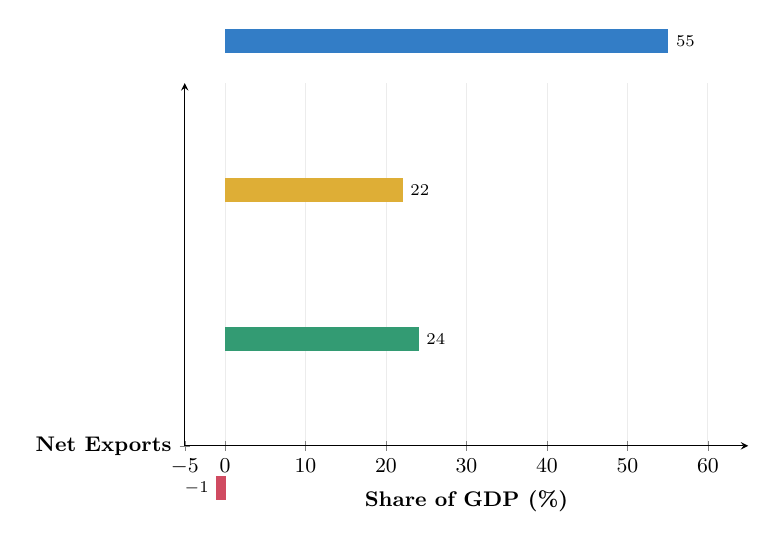
\begin{tikzpicture}[scale=0.85]
  \begin{axis}[
    xbar,
    width=10cm, height=7cm,
    xlabel={\textbf{Share of GDP (\%)}},
    symbolic y coords={Net Exports, Investment, Government, Consumption},
    ytick=data,
    yticklabel style={font=\small\bfseries},
    xmin=-5, xmax=65,
    xtick={-5,0,10,20,30,40,50,60},
    tick label style={font=\small},
    label style={font=\small\bfseries},
    axis lines=left,
    grid=major, grid style={gray!15},
    nodes near coords,
    nodes near coords style={font=\scriptsize},
    clip=false,
  ]
  \addplot[fill=canadared!80, draw=canadared!80]
    coordinates {(-1,{Net Exports})};
  \addplot[fill=leafgreen!80, draw=leafgreen!80]
    coordinates {(24,{Investment})};
  \addplot[fill=goldenrod!90, draw=goldenrod!90]
    coordinates {(22,{Government})};
  \addplot[fill=accent!80, draw=accent!80]
    coordinates {(55,{Consumption})};
  \end{axis}
\end{tikzpicture}
\end{center}
{\scriptsize\itshape Source: Statistics Canada, CANSIM 36-10-0121-01 (2023). Shares are approximate and rounded.}
\end{frame}

\begin{frame}{Value Added: An Alternative Way to Calculate GDP}
\transfade
\begin{itemize}[<+->]
  \item \textbf{Value added} at each stage of production = the firm's revenue minus the cost of intermediate inputs purchased from other firms.
  \item Summing value added across all firms gives total GDP.
  \item \textbf{Example (Canadian lumber to furniture):}
  \begin{itemize}[<+->]
    \item Timber harvester sells logs for \$200; value added = \$200.
    \item Sawmill buys logs (\$200), sells lumber for \$350; value added = \$150.
    \item Furniture maker buys lumber (\$350), sells chair for \$500; value added = \$150.
    \item \textbf{Total value added = \$500 = final sale price.}
  \end{itemize}
\end{itemize}
\end{frame}

% ============================================================
\section{4.2 Does GDP Measure What We Want?}
% ============================================================

\begin{frame}{4.2 Learning Objective}
\transfade
\begin{block}{Goal}
Discuss whether GDP is a good measure of well-being.
\end{block}
\begin{itemize}[<+->]
  \item GDP is a useful measure of total output.
  \item But it has \textbf{shortcomings} both as a measure of total production and as a measure of well-being.
\end{itemize}
\end{frame}

\begin{frame}{What GDP Misses: Production Gaps}
\transfade
\begin{itemize}[<+->]
  \item \textbf{Household production}: childcare, cooking, home repairs --- if done at home, not counted in GDP; if hired out, they are counted.
  \begin{itemize}[<+->]
    \item Statistics Canada's Household Satellite Account estimates household production was worth $\approx$\$460B (41\% of GDP) in 2015.
  \end{itemize}
  \item \textbf{Informal (shadow) economy}: unreported legal activities and illegal transactions.
  \begin{itemize}[<+->]
    \item Estimated at $\approx$\textbf{13\%} of official Canadian GDP --- real value created but not captured.
  \end{itemize}
\end{itemize}
\end{frame}

\begin{frame}{What GDP Misses: Well-Being Gaps}
\transfade
\begin{itemize}[<+->]
  \item Even perfect GDP misses key dimensions of well-being:
  \begin{itemize}[<+->]
    \item \textbf{Leisure:} Canadians work $\approx$1,700 hours/year vs.\ the OECD average of 1,752 --- leisure has real value.
    \item \textbf{Pollution:} oilsands extraction raises GDP but degrades air and water quality; the cleanup cost is also GDP.
    \item \textbf{Income distribution:} GDP per capita was $\approx$\$57,000 in 2023, but the Gini coefficient shows significant inequality.
    \item \textbf{Crime and social problems:} more policing raises GDP even though the underlying problem is bad.
  \end{itemize}
\end{itemize}
\end{frame}

\begin{frame}{GDP and Well-Being: The Bottom Line}
\transfade
\begin{itemize}[<+->]
  \item GDP is an \alert{imperfect} but \textbf{useful} indicator:
  \begin{itemize}[<+->]
    \item Higher GDP per person is strongly correlated with higher life expectancy, education, and happiness measures.
    \item Canada's GDP per capita $\approx$\$57,000 (2023) puts it among the top 20 worldwide (World Bank).
  \end{itemize}
  \item Alternatives being developed:
  \begin{itemize}[<+->]
    \item \textbf{OECD Better Life Index} (Canada ranks \#5 overall, 2024).
    \item \textbf{Statistics Canada's Quality of Life Framework} (launched 2021): 84 indicators across 5 domains.
    \item \textbf{UN Human Development Index:} combines income, education, and life expectancy.
  \end{itemize}
\end{itemize}
\end{frame}

% ============================================================
\section{4.3 Real GDP versus Nominal GDP}
% ============================================================

\begin{frame}{4.3 Learning Objective}
\transfade
\begin{block}{Goal}
Discuss the difference between real GDP and nominal GDP.
\end{block}
\begin{itemize}[<+->]
  \item GDP is measured in dollars --- but dollar values change when prices change.
  \item We must separate \textbf{quantity changes} from \textbf{price changes}.
  \item \textbf{Nominal GDP:} values final output at \alert{current-year prices}.
  \item \textbf{Real GDP:} values final output at \alert{base-year prices} (Statistics Canada uses 2017 as reference year).
\end{itemize}
\end{frame}

%--- Fig 4.3: Real vs Nominal GDP Canada ---
\begin{frame}{Figure 4.3 -- Nominal vs.\ Real GDP: Canada 2012--2024}
\begin{center}
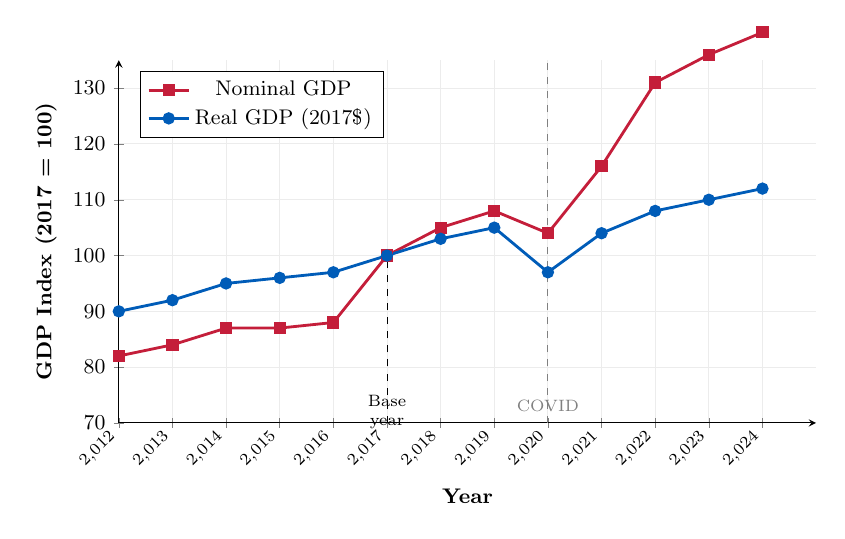
\begin{tikzpicture}[scale=0.85]
  \begin{axis}[
    width=12cm, height=7cm,
    xlabel={\textbf{Year}},
    ylabel={\textbf{GDP Index} (2017 = 100)},
    xmin=2012, xmax=2025,
    ymin=70, ymax=135,
    xtick={2012,2013,2014,2015,2016,2017,2018,2019,2020,2021,2022,2023,2024},
    xticklabel style={rotate=45, anchor=east, font=\scriptsize},
    ytick={70,80,90,100,110,120,130},
    tick label style={font=\small},
    label style={font=\small\bfseries},
    axis lines=left,
    grid=major, grid style={gray!15},
    legend pos=north west,
    legend style={font=\small},
    clip=false,
  ]
  % Nominal GDP index (2017=100): rises faster due to inflation
  \addplot[very thick, color=canadared, mark=square*, mark size=2pt]
    coordinates {
      (2012,82)(2013,84)(2014,87)(2015,87)(2016,88)
      (2017,100)(2018,105)(2019,108)(2020,104)(2021,116)
      (2022,131)(2023,136)(2024,140)
    };
  \addlegendentry{Nominal GDP}
  % Real GDP index (2017=100): slower growth
  \addplot[very thick, color=accent, mark=*, mark size=2pt]
    coordinates {
      (2012,90)(2013,92)(2014,95)(2015,96)(2016,97)
      (2017,100)(2018,103)(2019,105)(2020,97)(2021,104)
      (2022,108)(2023,110)(2024,112)
    };
  \addlegendentry{Real GDP (2017\$)}
  % Annotate COVID dip
  \draw[dashed, color=gray] (axis cs:2020,70) -- (axis cs:2020,135);
  \node[font=\scriptsize, text=gray, align=center] at (axis cs:2020,73)
    {COVID};
  % Base year annotation
  \draw[dashed, color=black] (axis cs:2017,70) -- (axis cs:2017,101);
  \node[font=\scriptsize, align=center] at (axis cs:2017,72) {Base\\year};
  \end{axis}
\end{tikzpicture}
\end{center}
{\scriptsize\itshape Source: Statistics Canada, CANSIM 36-10-0104-01. Approximate index values.}
\end{frame}

\begin{frame}{Calculating Real GDP: A Simple Example}
\transfade
\small
\begin{itemize}[<+->]
  \item Suppose Canada produces only two goods: lumber and canola oil.
\end{itemize}
\vspace{0.3em}
\renewcommand{\arraystretch}{1.3}
\begin{tabular}{lcccc}
\toprule
 & \multicolumn{2}{c}{\textbf{Base Year (2017)}} & \multicolumn{2}{c}{\textbf{Current Year (2023)}} \\
\cmidrule(lr){2-3}\cmidrule(lr){4-5}
\textbf{Good} & Price & Qty & Price & Qty \\
\midrule
Lumber (M$\text{m}^3$) & \$100 & 10 & \$130 & 12 \\
Canola oil (Mt) & \$500 & 5 & \$650 & 6 \\
\midrule
\textbf{Nominal GDP} & \multicolumn{2}{c}{\$3,500} & \multicolumn{2}{c}{\textcolor{canadared}{\$5,460}} \\
\textbf{Real GDP (2017\$)} & \multicolumn{2}{c}{\$3,500} & \multicolumn{2}{c}{\textcolor{accent}{\$4,200}} \\
\bottomrule
\end{tabular}
\begin{itemize}[<+->]
  \item Nominal GDP overstates growth by counting higher prices.
  \item Real GDP isolates the increase in \textbf{actual quantities produced}.
\end{itemize}
\end{frame}

\begin{frame}{Interpreting Real GDP}
\transfade
\begin{itemize}[<+->]
  \item In the base year, real and nominal GDP are \textbf{equal by definition}.
  \item After the base year:
  \begin{itemize}[<+->]
    \item If prices rise: nominal GDP grows \alert{faster} than real GDP.
    \item If prices fall: nominal GDP grows \alert{slower} than real GDP.
  \end{itemize}
  \item Growth rates reported in the news refer to \textbf{real GDP growth}.
  \item Statistics Canada uses \textbf{chain-weighted} prices (not a fixed basket) to avoid distortions as relative prices change over time.
\end{itemize}
\end{frame}

%--- GDP Deflator ---
\begin{frame}{The GDP Deflator}
\transfade
\begin{itemize}[<+->]
  \item The \textbf{GDP deflator} measures the overall price level of all final goods and services:
  \[
    \text{GDP Deflator} = \frac{\text{Nominal GDP}}{\text{Real GDP}} \times 100
  \]
  \item In the base year: GDP Deflator = 100.
  \item \textbf{Canadian example:}
  \begin{itemize}[<+->]
    \item 2023: Nominal GDP $\approx$\$2,890B; Real GDP (2017\$) $\approx$\$2,160B.
    \[
      \text{Deflator}_{2023} = \frac{2{,}890}{2{,}160} \times 100 \approx 133.8
    \]
    \item This means the overall price level rose $\approx$33.8\% since 2017.
  \end{itemize}
\end{itemize}
\end{frame}

% ============================================================
\section{4.4 Other Measures of Total Production and Income}
% ============================================================

\begin{frame}{Other Measures of Total Production and Income}
\transfade
\begin{itemize}[<+->]
  \item Beyond GDP, national accounts construct:
  \begin{itemize}[<+->]
    \item \textbf{Gross National Income (GNI):} GDP plus net income earned by Canadians abroad minus income earned by foreigners in Canada.
    \item \textbf{National Income:} GNI minus depreciation.
    \item \textbf{Personal Income:} income received by households, including government transfers.
    \item \textbf{Disposable Personal Income:} personal income minus taxes paid.
  \end{itemize}
  \item \textbf{Canadian fact:} Canada's GNI is close to GDP since income flows in and out roughly balance.
  \item These measures are useful when studying \textbf{household budgets} and \textbf{living standards}.
\end{itemize}
\end{frame}

% ============================================================
\section*{Chapter Summary}
% ============================================================

\begin{frame}{Things to Remember}
\transfade
\begin{itemize}[<+->]
  \item GDP counts \textbf{final} goods and services only --- to avoid double-counting intermediate inputs.
  \item GDP measures production \textbf{within borders} --- not by whom the company is owned.
  \item \textbf{Total production = total income} --- the circular-flow identity.
  \item \textbf{Real GDP} removes inflation; \textbf{nominal GDP} does not --- always use real for quantity comparisons.
  \item GDP is a useful but imperfect proxy for well-being --- it misses household production, leisure, inequality, and environmental quality.
\end{itemize}
\end{frame}

\begin{frame}{Chapter Summary}
\transfade
\begin{itemize}[<+->]
  \item \textbf{GDP} = market value of all final goods and services produced in Canada during a period.
  \item Measured two ways (both yield the same answer): \textbf{income approach} and \textbf{expenditure approach} ($Y = C + I + G + NX$).
  \item GDP omits household production ($\approx$41\% of GDP) and the shadow economy ($\approx$13\% of GDP).
  \item \textbf{Real GDP} controls for inflation using base-year prices; Statistics Canada uses chain-weighting.
  \item The \textbf{GDP deflator} = (Nominal/Real) $\times$ 100 measures overall price level.
  \item Other measures: GNI, National Income, Personal Income, Disposable Income.
\end{itemize}
\end{frame}

\begin{frame}
\centering
\Huge \textbf{Thank you!}\\[1em]
\normalsize Questions?\\[0.5em]
\small\itshape Data: Statistics Canada CANSIM 36-10-0104-01, 36-10-0121-01; World Bank; OECD Better Life Index 2024
\end{frame}

\end{document}
